\documentclass[10pt]{extarticle}
\usepackage{etoolbox}
\AtBeginEnvironment{tabular}{\fontsize{9}{11}\selectfont}
\usepackage[most]{tcolorbox}
\usepackage[colorlinks=true, linkcolor=black, urlcolor=blue]{hyperref}
\usepackage{graphicx}
\usepackage[utf8]{inputenc}
\DeclareUnicodeCharacter{221B}{\ensuremath{\sqrt[3]{}}} % Map ∛ to cube-root
\usepackage{xcolor}
\definecolor{mpgDarkGreen}{HTML}{005555}
\definecolor{mpgLightGreen}{HTML}{006c66}
\definecolor{mpgDarkGrey}{HTML}{777777}
\definecolor{mpgAccentOrange}{HTML}{ef7c00}
\definecolor{mpgAccentGreen}{HTML}{c6d325}
\definecolor{mpgAccentBlue}{HTML}{29485d}
\definecolor{mpgAccentCyan}{HTML}{00b1ea}
\usepackage[a4paper, left=2.5cm, right=2.5cm, top=2.5cm, bottom=2.5cm]{geometry}
\usepackage{setspace}
\setstretch{1.5}
\usepackage{titlesec}

\renewcommand{\figurename}{Fig.}
\renewcommand{\thefigure}{\arabic{figure}\,\textbar}
\usepackage{caption}
\DeclareCaptionFont{figfont}{\fontsize{9}{11}\selectfont}
\captionsetup[figure]{labelfont={bf,figfont}, textfont=figfont, labelsep=space}

\usepackage{enumitem} % for description formatting

\titleformat{\section}
  {\color{mpgDarkGreen}\normalfont\fontsize{16}{18}\selectfont\bfseries}
  {\thesection}{1em}{}

\titleformat{\subsection}
  {\color{mpgLightGreen}\normalfont\fontsize{14}{16}\selectfont\bfseries}
  {\thesubsection}{1em}{}

\titleformat{\subsubsection}
  {\color{mpgLightGreen}\normalfont\fontsize{12}{14}\selectfont\bfseries}
  {\thesubsubsection}{1em}{}

\usepackage{listings}
\lstset{
    basicstyle=\color{black}\fontsize{9}{11}\selectfont\ttfamily,
    backgroundcolor=\color{gray!20},
    frame=single,
    rulecolor=\color{black},
    breaklines=true
}
\usepackage{pdfpages}
\usepackage[sfdefault]{roboto}
\renewcommand*\familydefault{\sfdefault}
\setlength{\parindent}{0pt}
\usepackage{hyperref}
\usepackage{longtable}
\usepackage{fancyhdr}
\pagestyle{fancy}
\fancyhf{} % clear all headers and footers
\fancyhead[R]{\textsf{\nouppercase{\leftmark}}}
\fancyfoot[C]{\textsf{\thepage}} 
\renewcommand{\headrulewidth}{0.4pt}
\renewcommand{\footrulewidth}{0pt}
% Make each new section start on a new page.
\let\oldsection\section
\renewcommand{\section}[1]{\clearpage\oldsection{#1}}
\begin{document}

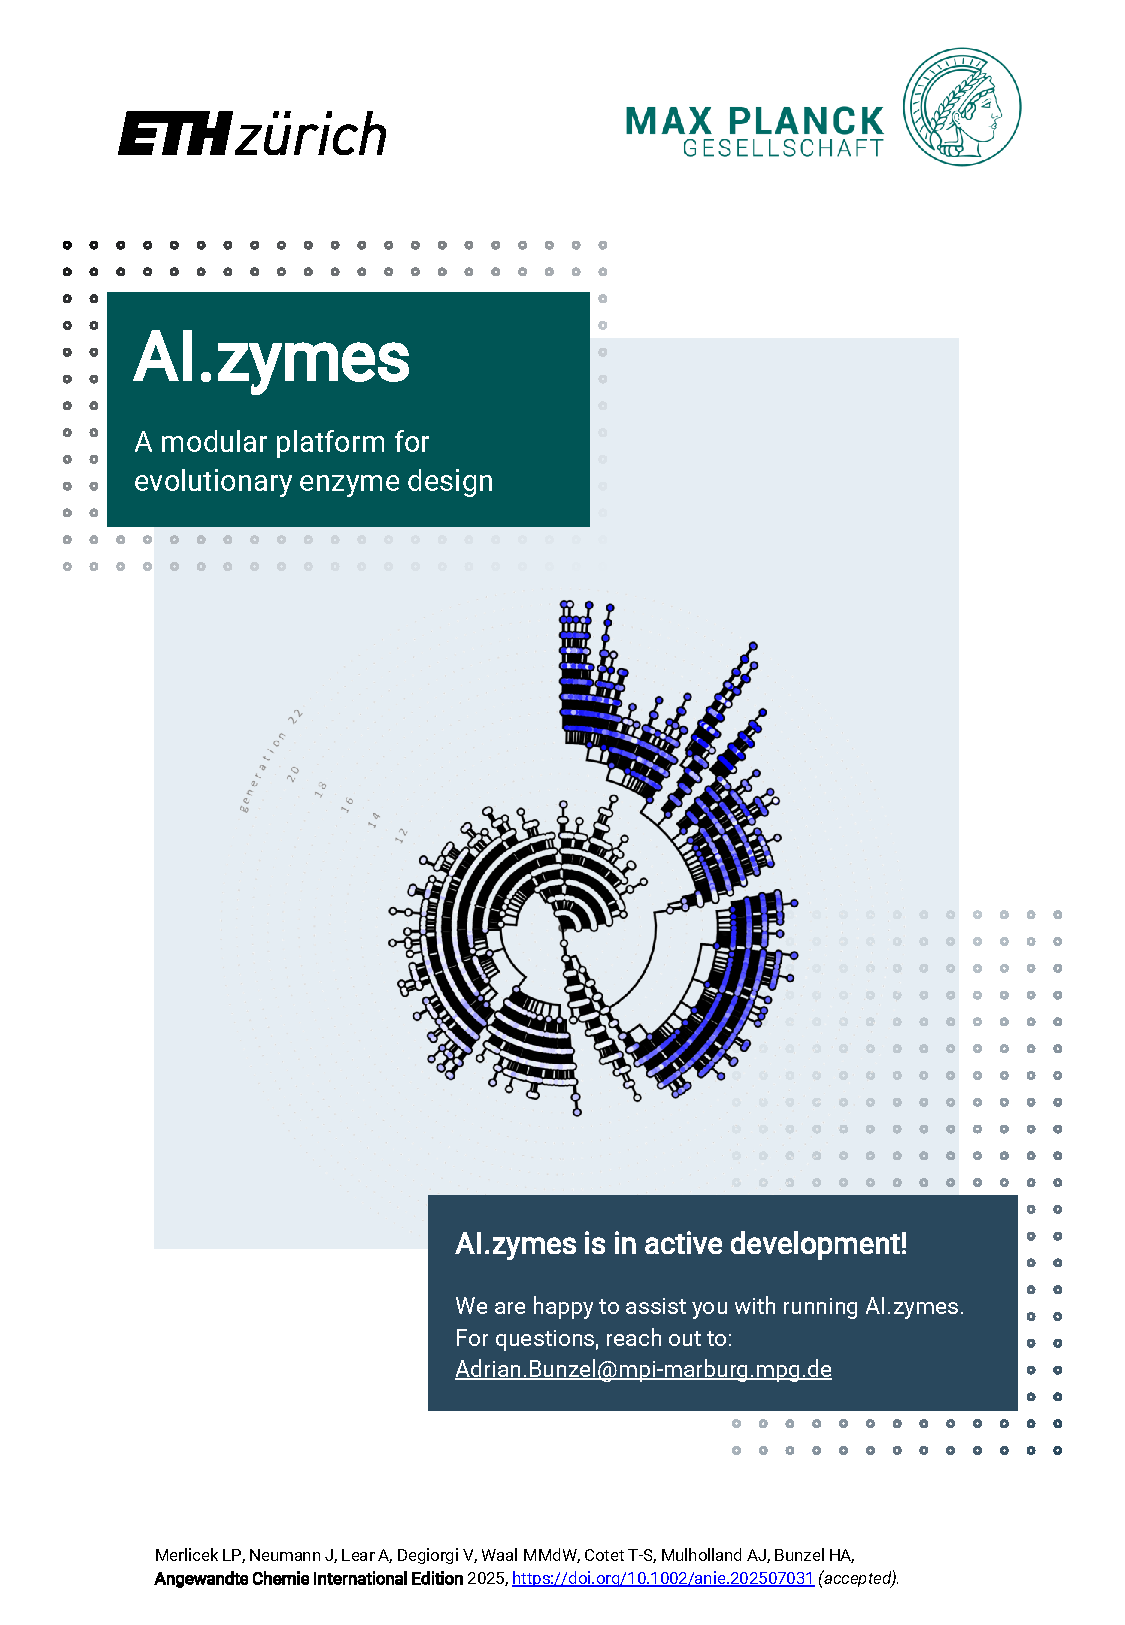
\includepdf[pages=1]{cover.pdf}
\clearpage
\pagenumbering{roman}
\setcounter{page}{1}

\clearpage\pagenumbering{roman}\setcounter{page}{1}
% Temporarily restore the original section command for the TOC
\let\sectionTemp=\section
\let\section=\oldsection
\clearpage
{\setstretch{1.15}\tableofcontents}
\clearpage
\let\section=\sectionTemp

\clearpage\pagenumbering{arabic}\setcounter{page}{1}
\section{Installation}

We recommend installing AI.zymes with pip. For code development, AI.zymes can also be cloned from the GitHub repository. To install AI.zymes with pip, run:

\vspace*{0.5\baselineskip}
\begin{lstlisting}[basicstyle=\color{black}\fontsize{9}{11}\selectfont\ttfamily, frame=single, rulecolor=\color{black}, breaklines=true]
pip install aizymes
\end{lstlisting}
\vspace*{0.5\baselineskip}

AI.zymes works by wrapping around various bioengineering tools that need to be installed seperately. A list of all established tools in AI.zymes is given in the section \textbf{Available Tools}. For some of these tools, their paths need to be defined to connect with them. To that end, AI.zymes will create a \textbf{.config} file when you run AIzymes for first time. 

\begin{tcolorbox}[colback=mpgAccentBlue!20!white,colframe=mpgAccentBlue!80!black,title=Note]
Several tools, such as Rosetta, need to be installed seperately. See \textbf{Available Tools} for guidelines on how to find the installation instructions.
\end{tcolorbox}

\begin{tcolorbox}[colback=mpgAccentOrange!20!white,colframe=mpgAccentOrange!80!black,title=Warning]
AI.zymes currently only works with SLURM.
If you want to use a different submission system, please contact Adrian.Bunzel@mpi-marburg.mpg.de.
\end{tcolorbox}

\subsection{Installation via GitHub}

To install AI.zymes via GitHub, clone the repository, create the AI.zymes python environment, and add the repository to your pythonpath. To clone AI.zyme, run:

\vspace*{0.5\baselineskip}
\begin{lstlisting}[basicstyle=\color{black}\fontsize{9}{11}\selectfont\ttfamily, frame=single, rulecolor=\color{black}, breaklines=true]
git clone https://github.com/bunzela/AIzymes.git
\end{lstlisting}
\vspace*{0.5\baselineskip}

You can either create your own AI.zymes environment, or install all required packages in your existing environment.

\vspace*{0.5\baselineskip}
\begin{lstlisting}[basicstyle=\color{black}\fontsize{9}{11}\selectfont\ttfamily, frame=single, rulecolor=\color{black}, breaklines=true]
cd AIzymes
# To build new environemnt
conda env create -f environment.yml --name AIzymes 
# Alternative to install packages in curent environemnt:
# conda env update -f environment.yml --prune
\end{lstlisting}
\vspace*{0.5\baselineskip}

Add the path to AI.zymes to your .bashrc. Replace \textbf{PATH\_TO\_AIZYMES} with the corect path to AI.zymes.

\vspace*{0.5\baselineskip}
\begin{lstlisting}[basicstyle=\color{black}\fontsize{9}{11}\selectfont\ttfamily, frame=single, rulecolor=\color{black}, breaklines=true]
echo 'export PYTHONPATH="$PYTHONPATH:PATH_TO_AIZYMES/src/aizymes"' >> ~/.bashrc
source ~/.bashrc
\end{lstlisting}
\vspace*{0.5\baselineskip}\section{Quick Start}

\begin{tcolorbox}[colback=mpgAccentCyan!20!white,colframe=mpgAccentCyan!80!black,title=Tip]
Get started with AI.zymes using the notebook \textbf{example\_notebooks/Example\_KSI.ipynb}.
\end{tcolorbox}

The notebook \textbf{Example\_KSI.ipynb} can be used to improve the promoscious Kemnp eliminase activity of KSI. Here, each step of this notebook is explained briefly. For detailed instructions on how to use AI.zymes, check \textbf{5. Full Manual}.

\subsection{Create an Instance of the AI.zymes class}

To start AI.zymes, you first need to create an Instance of the AI.zymes class and set \textbf{FOLDER\_HOME}.
All data generated during the AI.zymes run are storred in \textbf{FOLDER\_HOME}.
Asides from the design structures, \textbf{FOLDER\_HOME} contains information on the settings chosen during design (\textbf{variables.json})
and a database containing the sequences and scores of all designs (\textbf{all\_scores.csv}).

\vspace*{0.5\baselineskip}
\begin{lstlisting}[basicstyle=\color{black}\fontsize{9}{11}\selectfont\ttfamily, frame=single, rulecolor=\color{black}, breaklines=true]
# Import AI.zymes
from aizymes import * 
         
# Create instance of AIzymes_MAIN
AIzymes = AIzymes_MAIN(FOLDER_HOME = 'Example_KSI') 
\end{lstlisting}
\vspace*{0.5\baselineskip}

\subsection{Set up AI.zymes for design}

Befor starting design, the basic folder structure and input files need to be set up with \textbf{AIzymes.setup}. The input settings used here are discussed in detail in \textbf{5. Full Manual}.

\begin{tcolorbox}[colback=mpgAccentGreen!20!white,colframe=mpgAccentGreen!80!black,title=Important]
All inputfiles provided need to be in the folder \textbf{Input} in the same directory as where you running the code.
Note that structures can also be loaded from a different folder using \textbf{FOLDER\_PAR\_STRUC}.
\end{tcolorbox}

\begin{tcolorbox}[colback=mpgAccentBlue!20!white,colframe=mpgAccentBlue!80!black,title=Note]
If the config file specified with \textbf{SYSTEM} does not exist,
\textbf{AIzymes.setup} will prompt for inputs to generate a new config file.
The config file contains system-specific information neccesary to run AI.zymes.
\end{tcolorbox}

\begin{tcolorbox}[colback=mpgAccentOrange!20!white,colframe=mpgAccentOrange!80!black,title=Warning]
AI.zymes currently only works with SLURM.
If you want to use a different submission system, please contact Adrian.Bunzel@mpi-marburg.mpg.de.
\end{tcolorbox}

\vspace*{0.5\baselineskip}
\begin{lstlisting}[basicstyle=\color{black}\fontsize{9}{11}\selectfont\ttfamily, frame=single, rulecolor=\color{black}, breaklines=true]
AIzymes.setup(
# General Design Settings
    WT                = "1ohp",
    LIGAND            = "5TS",
    DESIGN            = "11,14,15,18,38,54,55,58,63,65,80,82,84,97,99,101,112,114,116",
    PARENT_DES_MED    = ['RosettaDesign',
                         'ESMfold','MDMin','RosettaRelax','ElectricFields'],
    DESIGN_METHODS    = [[0.5,'SolubleMPNN',\
                              'ESMfold','MDMin','RosettaRelax','ElectricFields'],\
                         [0.5,'RosettaDesign',\
                              'ESMfold','MDMin','RosettaRelax','ElectricFields']],
# General Scoring Settings    
    SELECTED_SCORES   = ["total","catalytic","interface","efield", "identical"],    
# General Job Settings
    MAX_JOBS          = 72,
    MAX_GPUS          = 4,
    MEMORY            = 450,
    N_PARENT_JOBS     = 144,
    MAX_DESIGNS       = 5000,
    KBT_BOLTZMANN     = [1.0, 0.5, 0.02],   
    SUBMIT_PREFIX     = "KSI_TEST", 
    SYSTEM            = "AIzymes.config",
# RosettaDesign Settings
    CST_NAME          = "5TS_enzdes_planar_tAB100", 
    CST_DIST_CUTOFF   = 40.,
# FieldTools settings
    FIELD_TARGET      = ":5TS@C9 :5TS@H04",
 )                     
\end{lstlisting}
\vspace*{0.5\baselineskip}

\subsection{Submit controller to run AI.zymes}

Once the setup is completet you need to start the controller.
\textbf{AIzymes.submit\_controller()} will launch am HPC job that runs the controller.

\vspace*{0.5\baselineskip}
\begin{lstlisting}[basicstyle=\color{black}\fontsize{9}{11}\selectfont\ttfamily, frame=single, rulecolor=\color{black}, breaklines=true]
AIzymes.submit_controller()
\end{lstlisting}
\vspace*{0.5\baselineskip}

\begin{tcolorbox}[colback=mpgAccentCyan!20!white,colframe=mpgAccentCyan!80!black,title=Tip]
You can check the progress of AI.zymes and trouble-shoot errors with the controller.log.
Alternatively, you can also check the output and errors of individual designs.
\end{tcolorbox}

\vspace*{0.5\baselineskip}
\begin{lstlisting}[basicstyle=\color{black}\fontsize{9}{11}\selectfont\ttfamily, frame=single, rulecolor=\color{black}, breaklines=true]
!tail -n 50 {FOLDER_HOME}/controller.log
!ls {FOLDER_HOME}/designs/0/scripts
\end{lstlisting}
\vspace*{0.5\baselineskip}

\subsection{Analysis tools to check AI.zymes}

AI.zymes comes with several tools to analyze the design runs. Use \textbf{AIzymes.plot} to create a range of plots, showing how the scores evolved over time.
Alternatively, you can use \textbf{AIzymes.print\_statistics()} to print out key information from the \textbf{all\_scores.csv} file.


\begin{tcolorbox}[colback=mpgAccentBlue!20!white,colframe=mpgAccentBlue!80!black,title=Note]
\textbf{NORM} is used to ensure comarability between design runs by normalizing all results to the same values.
\end{tcolorbox}

\vspace*{0.5\baselineskip}
\begin{lstlisting}[basicstyle=\color{black}\fontsize{9}{11}\selectfont\ttfamily, frame=single, rulecolor=\color{black}, breaklines=true]
AIzymes.plot(NORM = {
                'total_score': [310, 380], 
                'catalytic_score': [-30, -4],
                'interface_score': [20, 30],
                'final_score': [-30, 0],
                'efield_score': [-40, 30],
                'identical_score': [0, 1.05],
             })                   
\end{lstlisting}
\vspace*{0.5\baselineskip}

\begin{tcolorbox}[colback=mpgAccentCyan!20!white,colframe=mpgAccentCyan!80!black,title=Tip]
\textbf{AIzymes.print\_statistics()} can be very helpfull to trouble-shoot!
\end{tcolorbox}

\vspace*{0.5\baselineskip}
\begin{lstlisting}[basicstyle=\color{black}\fontsize{9}{11}\selectfont\ttfamily, frame=single, rulecolor=\color{black}, breaklines=true]
AIzymes.print_statistics()
\end{lstlisting}
\vspace*{0.5\baselineskip}

\subsection{Extract best structures after AI.zymes run}

Finally, to extract the hits from your AI.zymes run, execute \textbf{AIzymes.best\_structures()}

\begin{tcolorbox}[colback=mpgAccentBlue!20!white,colframe=mpgAccentBlue!80!black,title=Note]
Structures will be saved with their final score as prefix, helping to identify the best designs.
\end{tcolorbox}

\vspace*{0.5\baselineskip}
\begin{lstlisting}[basicstyle=\color{black}\fontsize{9}{11}\selectfont\ttfamily, frame=single, rulecolor=\color{black}, breaklines=true]
AIzymes.best_structures()      
\end{lstlisting}
\vspace*{0.5\baselineskip}\section{Available Tools}

AI.zymes works by wrapping around a range of bioengineering tools. While some of these tools can be readily installed using \textit{pip} or \textit{conda}, others need to be installed as stand-alone programs. Furthermore, some programs need to be registered in the \textbf{config} file genereatd during the first run of AI.zymes

\makebox[3.5cm][l]{Rosetta\dotfill} Protein design and relaxation \\        
\makebox[3.5cm][l]{LigandMPNN\dotfill} Protein design with ligands \\    
\makebox[3.5cm][l]{SolubleMPNN\dotfill} Protein design without ligands \\  
\makebox[3.5cm][l]{AlphaFold3\dotfill} Structure prediciton with ligands \\ 
\makebox[3.5cm][l]{ESMFold\dotfill} Structure prediciton without ligands \\
\makebox[3.5cm][l]{AmberTools\dotfill} Structure minimization \\
\makebox[3.5cm][l]{FieldTools\dotfill} Electric field calculation \\        
\makebox[3.5cm][l]{BioDC\dotfill} Redox Potential calculation \\

\subsection{Protein Design Tolls}

\subsubsection{Rosetta}

Rosetta is a comprehensive suite of software for physics-based macromolecular modeling and design. In AI.zymes, it is used for (1) structure relaxation and repacking, and (2) enzyme design.

\\ \textbf{Available at:} \href{https://rosettacommons.org/software/download/}{https://rosettacommons.org/software/download/}


\subsubsection{LigandMPNN}

LigandMPNN is a deep-learning design tool that focuses on optimizing protein–ligand interactions. Within AI.zymes, it can be integrated to tailor the active-site environment by adjusting residues that directly interact with the chemical transition state or substrate.

\\ \textbf{Available at:} \href{https://github.com/dauparas/LigandMPNN}{https://github.com/dauparas/LigandMPNN}


\subsubsection{SolubleMPNN and ProteinMPNN}

SolubleMPNN is a deep-learning design tool used to generate protein sequences that fold into a given structural scaffold, often enhancing the stability of the input structure in the process. In AI.zymes, ProteinMPNN is used to remodel the protein scaffold, focusing on regions away from the active site to improve stability without compromising enzyme activity.

\\ \textbf{Available at:} \href{https://github.com/dauparas/ProteinMPNN}{https://github.com/dauparas/ProteinMPNN}

\subsection{Structure Prediction Tools}

\subsubsection{AlphaFold3}

AlphaFold3 is a deep learning-based structure prediction tool that can include a range of small-molecule ligands during prediction. In AI.zymes, AlphaFold3 is used to predict the three-dimensional structure of designed enzymes, especially those bound to ligands such as heme.

\\ \textbf{Available at:} \href{https://github.com/google-deepmind/alphafold3}{https://github.com/google-deepmind/alphafold3}

\subsubsection{ESMFold}

ESMFold leverages large protein language models for structure prediction. It is usually faster than AlphaFold3 but cannot include small-molecule ligands. In AI.zymes, ESMFold is used in combination with RosettaRelax and MDMin to generate ligand-bound structural models. This combination offers a fast route to assess design variants for proper folding and active-site organization without the computational overhead of traditional methods.

\\ \textbf{Available at:} \href{https://github.com/facebookresearch/esm}{https://github.com/facebookresearch/esm}
\\ \textbf{Installed using:} pip install transformers fair-esm

\subsubsection{AmberTools}

AmberTools is a collection of programs for molecular mechanics and dynamics, which help parameterize molecules and perform energy calculations. In the context of AI.zymes, AmberTools is used to minimize enzyme–ligand complexes (MDMin).

\\ \textbf{Available at:} \href{https://ambermd.org/AmberTools.php}{https://ambermd.org/AmberTools.php}
\\ \textbf{Installed using:} conda install conda-forge::ambertools


\subsection{Scoring Tools}

\subsubsection{FieldTools}

FieldTools is a computational tool for calculating electric fields in and around enzyme active sites. Since electrostatic interactions can greatly influence enzyme catalysis, AI.zymes incorporates FieldTools to quantitatively assess the catalytic electric field along a target bond. This evaluation is integrated into the multi-objective scoring system, enabling selection of variants that not only stabilize the protein and its active site but also optimize the electric field for enhanced catalysis.

\\ \textbf{Available at:} \href{https://github.com/bunzela/FieldTools}{https://github.com/bunzela/FieldTools}

\begin{tcolorbox}[colback=mpgAccentBlue!20!white,colframe=mpgAccentBlue!80!black,title=Note]
FieldTools has been hard-coded into AI.zymes and does not need to be installed seperately.
\end{tcolorbox}

\subsubsection{BioDC}

Work in progress...\section{Introduction}
\subsection{Coding philosophy}
AI.zymes is a modular program that seamlessly combines computational methods for design, structure prediction, and machine learning in a coherent enzyme design workflow (Fig. 1). To that end, AI.zymes employs a controller function that orchestrates the design process. The controller collects information from the designs and stores them in a shared database, selects which variants to submit for design, and decides what type of design or structure prediction algorithms to run with the selected variant. The controller is designed to manage a user-defined number of parallel design jobs, automatically starting a new job as soon as a previous one is completed. 
 
\begin{figure}[htbp]
\centering
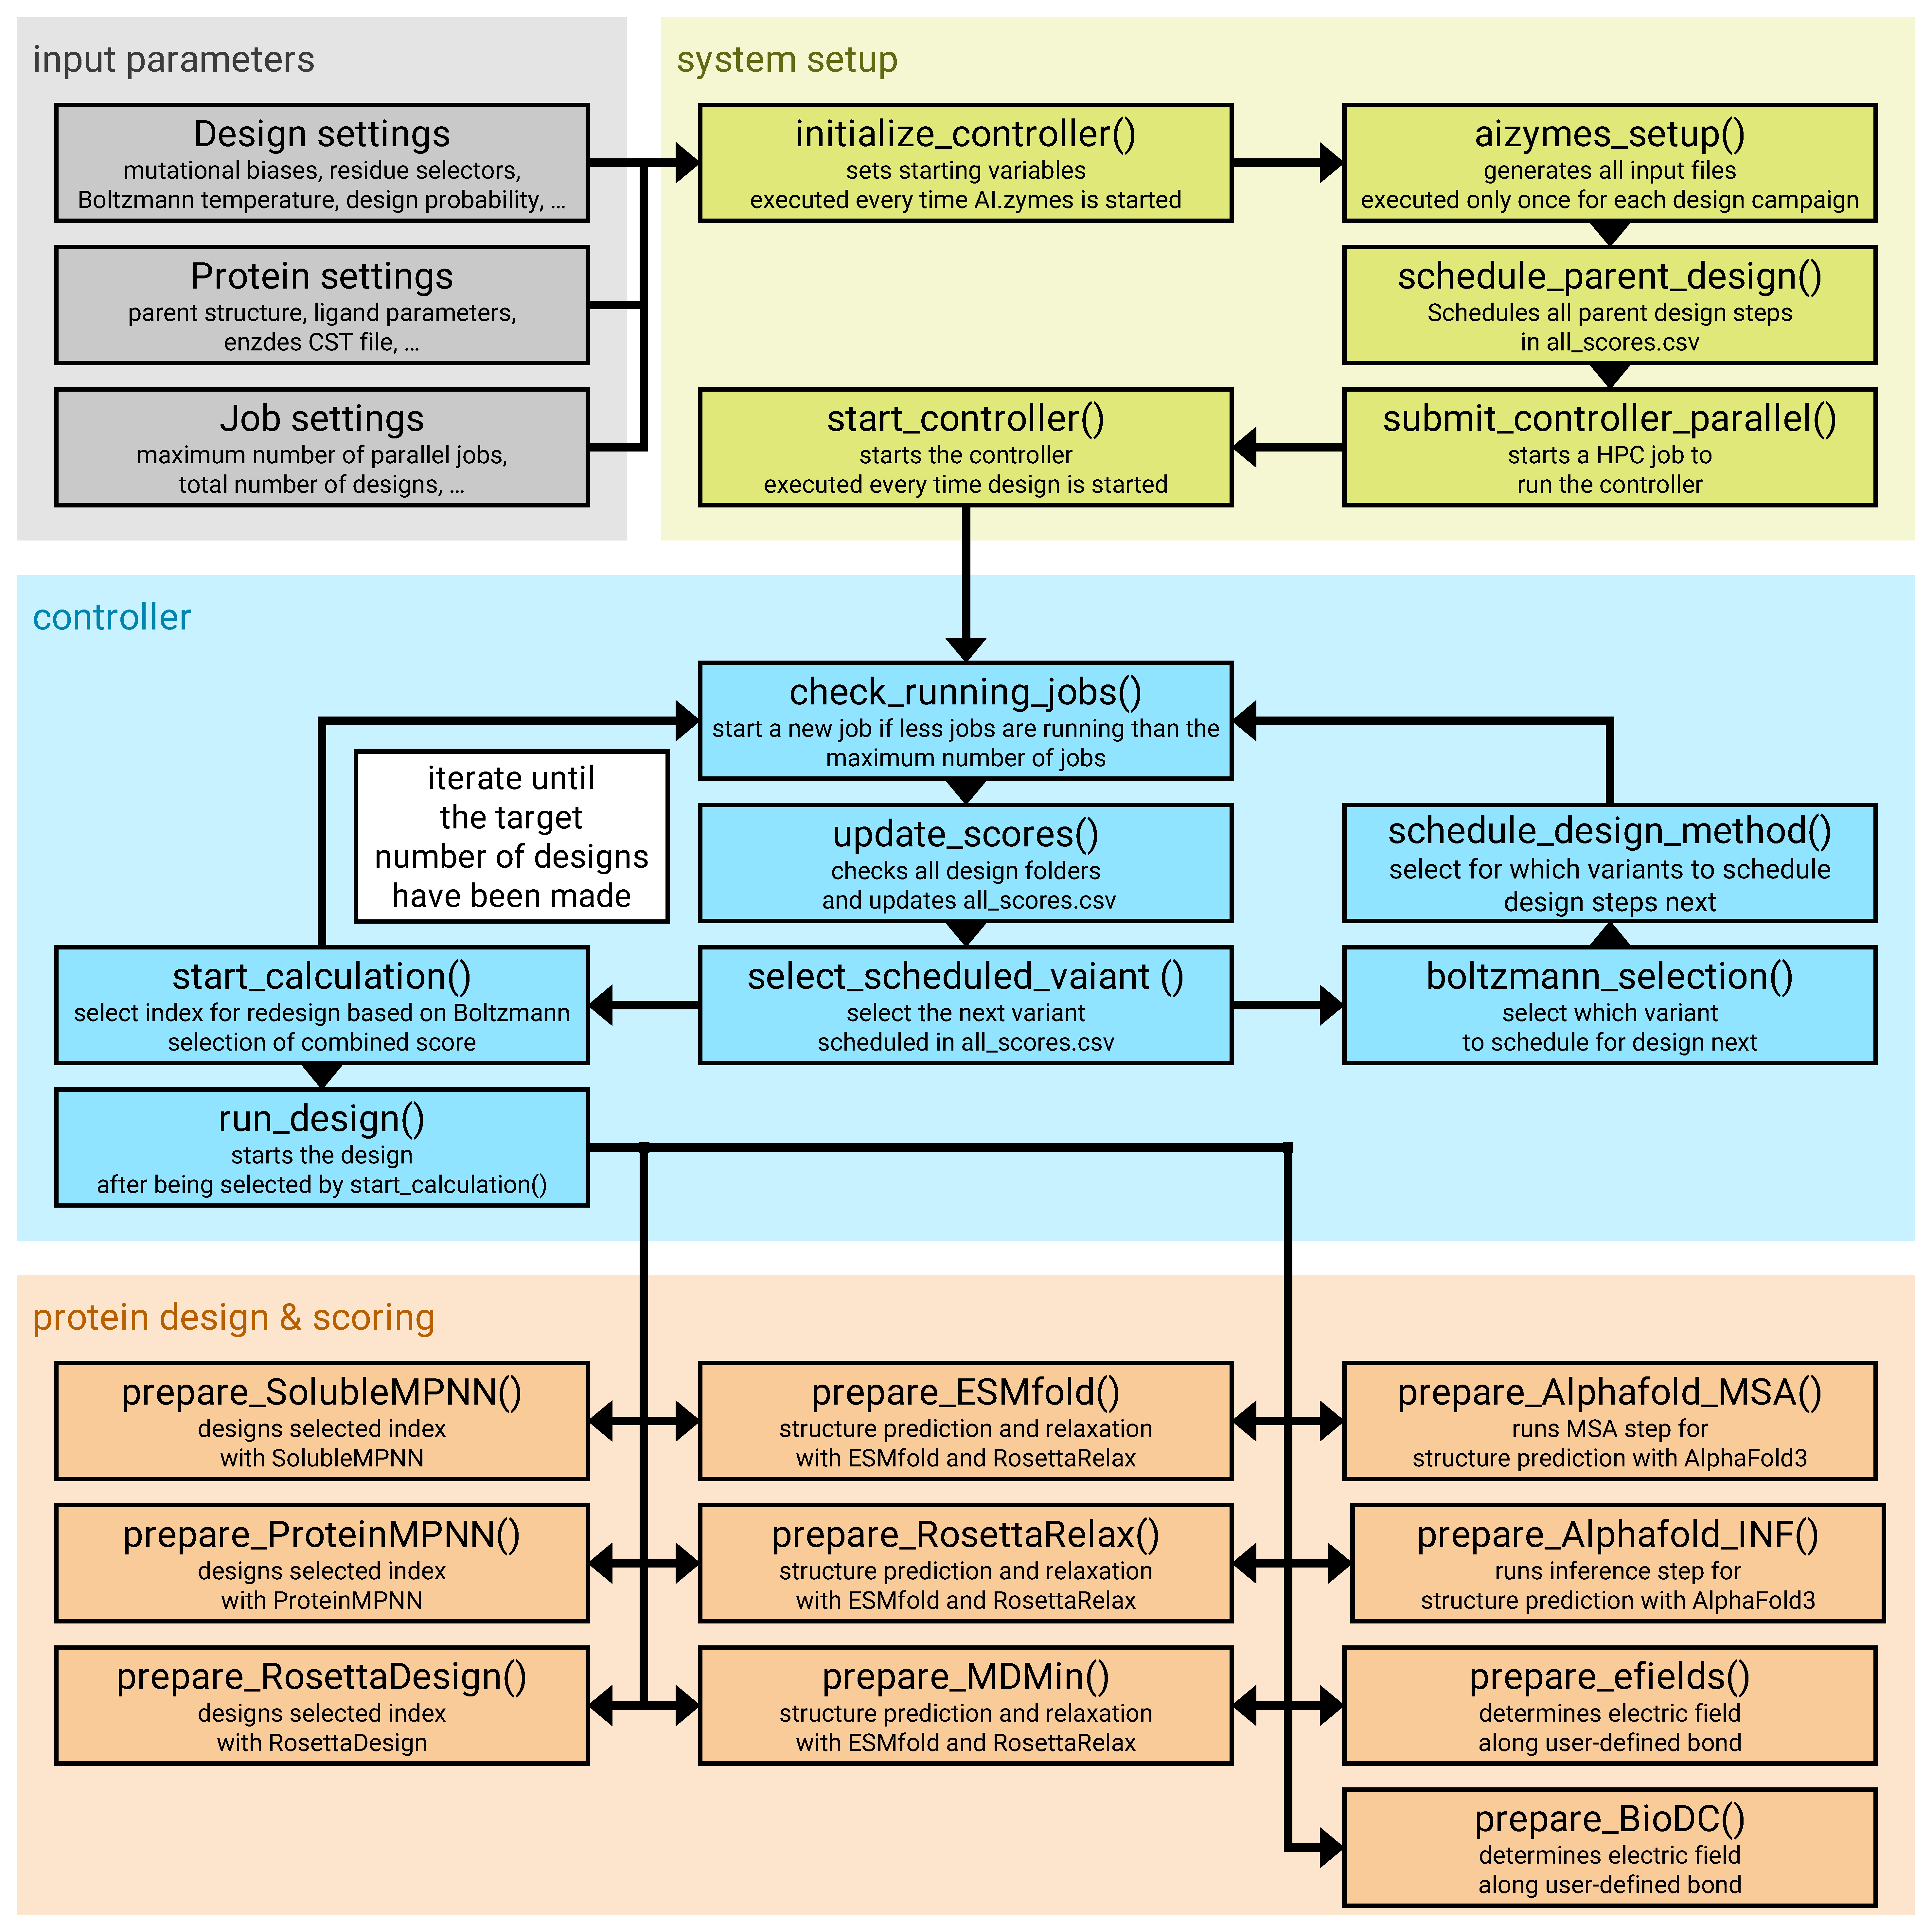
\includegraphics[width=16cm]{images/Figure1_AIzymes_Sheme.pdf}
\caption{\textbf{General Flow Chart of AI.zymes.} Based on a set of input variables (grey), AI.zymes will be set up and started (yellow). The main program of AI.zymes is the controller (blue), which controls the overall workflow, decides what action to take (salmon, red), and writes information into the databases (green).}
\end{figure}

\subsection{Basic concepts}

\subsubsection{Evolutionary "rounds" in AI.zymes}

The evolutionary algorithm in AI.zymes is not based on performing classical evolutionary rounds comprising mutagenesis and screening. Instead, the algorithm aims to maximize performance by constantly running a set number of design jobs set by \textbf{max\_jobs}. Whenever the number of running jobs falls below \textbf{max\_jobs}, AI.zymes spawns another design or structure prediction job. To choose the parent variant for design, AI.zymes performs multi-objective Boltzmann selection. Importantly, all designs are treated equally during Boltzmann selection, which selects from the growing pool of designs irrespective of which round the designs stemmed. Thus, design is not limited by a maximum number of rounds but a maximum number of designs (\textbf{max\_designs}).

\subsubsection{Scoring metrics}

AI.zymes employs various scoring metrics to assess various properties relevant to enzyme activity. The \textbf{total\_score} corresponds to the total energy of the system. This score reflects the \textbf{total\_score} of a structure in Rosetta and is referred to as "stability score" in the main text. The \textbf{interface\_score} corresponds to the binding energy of the ligand to the protein. This score was calculated using Rosetta's InterfaceScoreCalculator mover and is referred to as the "interface score" in AI.zymes. The \textbf{catalytic\_score} corresponds to the score of the catalytic interaction. It is calculated from the ideal interaction geometry described in a Rosetta\_Match constraint file format. Finally, the \textbf{efield\_score} describes the electric fields along the scissile C-H bond. Fields were calculated using FieldTools, and this score is referred to as the "electric field" in the main text.

Note that each variant in AI.zymes can have two sets of scores. All variants have scores from their initial design run. Variants selected for redesign also undergo structure prediction and relaxation, generating an updated set of scores. If available, Boltzmann selection is based on these updated scores; otherwise, the original design scores are used.

Furthermore, to run evolution in a forward-thinking manner, where the scores of the direct descendants of a variant can be included during screening, a metric called "potential" was introduced. The potential is the average of the score of the current variant and the scores of all its direct descendants.

\subsubsection{System startup}

To start AI.zymes, the system must be set up using \textbf{setup\_aizymes()} to create the overall file structure and stores all design-relevant parameters in the variables.json file. Among others, these include the name of the protein, ligand, and which residues can be designed. Furthermore, general settings can be set, such as how many jobs may run in parallel and how many designs will be made in total. Following the initial setup, \textbf{startup\_controller()} reads these parameters from the variables.json file and initializes all other required variables. Thus, \textbf{setup\_aizymes()} is only rone once, whereas \textbf{startup\_controller()} is executed every time the code is restarted. 

\subsubsection{Controller}

The controller is the central program of AI.zymes. It constantly cycles between the following steps:

1)	\textbf{check\_running\_jobs()} determines how many jobs are currently running on the system. If \textbf{MAX\_JOBS} are running, the controller sleeps for 20 s and rechecks the number of running jobs, or else the controller initiates a new design cycle.

2)	\textbf{update\_scores()} iterates through all designs and updates the \textbf{all\_scores.csv} database. \textbf{update\_scores()} also unblocks all indices for which the structure prediction runs are completed. 

3)	\textbf{check\_parent\_done()} checks if the initial non-evolutionary design for the parent variant has concluded. If fewer designs than N\_PARENT\_JOBS have been made, the controller skips the Boltzmann selection and instead runs \textbf{start\_parent\_design()}, starting a \textbf{run\_RosettaDesign()} job on the parent structure.

4)	\textbf{boltzmann\_selection()} initiates the Boltzmann selection to identify the next scaffold for design.

5)	\textbf{start\_calculation()} finally starts the design based on the selected input structure. \textbf{start\_calculation()} checks if there is a structure of the selected design that went through \textbf{ESMfold\_RosettaRelax()}. If not, the controller will start the structure prediction and block the selected index. If there is a relaxed structure, the controller will generate a new index into which the design will be stored. This involves creating a folder for the new design and appending the \textbf{all\_scores.csv} file with the selected index. To allow for a blend of design methods, the selected design will use \textbf{ProteinMPNN} instead of \textbf{RosettaDesign} with a user-defined probability \textbf{ProteinMPNN\_PROB}.

\subsubsection{Boltzmann selection}

In contrast to all other scores, the \textbf{catalytic\_score} has a clear minimum, with a score of zero reflecting a perfect agreement of the design with the target catalytic geometry. Thus, \textbf{catalytic\_score} was not included during Boltzmann selection but used as a binary cutoff to exclude variants before selection. To that end, the mean plus one standard deviation of the \textbf{catalytic\_score} of all designs is calculated, and all variants with a \textbf{catalytic\_score} below that cutoff are removed. Additionally, structures that are currently undergoing structure prediction are excluded from Boltzmann selection to prevent redundant structure prediction on the same structure.

Boltzmann selection is based on the design potentials and not on their scores. Boltzmann selection is performed on the combined\_potential, which is calculated from the average of the z-score standardized \textbf{total\_potential}, \textbf{interface\_potential}, and \textbf{efield\_potential}. Note that during normalization, potentials for which lower values are better are inverted (\textbf{total\_potential} and \textbf{interface\_potential}). Thus, higher combined\_potentials correspond to better variants. Boltzmann selection is performed at a user-defined temperature kbt\_boltzmann. To increase selection stringency during design, kbt\_boltzmann decreases with each new design from an initial \textbf{KBT\_BOLTZMANN} value with a \textbf{KBT\_BOLTZMANN\_DECAY} rate in a single exponential decay.
Boltzmann selection

\subsubsection{Database}

The all\_scores.csv database is the primary file containing all information from an AI.zymes run. Among other details, the database includes data on the specific settings for making each design and its resulting scores. Additionally, \textbf{all\_scores.csv} keeps track of which structures are currently undergoing structure prediction and are therefore excluded from Boltzmann selection. This exclusion prevents redundant structure prediction from being performed multiple times on the same structure.

\subsection{Available Modules in AI.zymes}

Currently, AI.zymes has established \textbf{run\_RosettaDesign()} and \textbf{run\_ProteinMPNN()} for design. For structure prediction and scoring, \textbf{run\_ESMfold\_RosettaRelax()} and \textbf{calc\_efields\_score()} have been established. Importantly, AI.zymes is built highly modularly, facilitating the future addition of other protein engineering packages to augment the computational evolution algorithm.

\subsubsection{Design with RosettaDesign}

\textbf{run\_RosettaDesign()} setups and submits a RosettaDesign run for the selected index based on RosettaScripts. AI.zymes dynamically generates the input .xml files that control RosettaScripts. An example .xml file can be found in 6.4 Example .xml file for RosettaDesign. Briefly, a geometry bias from the RosettaMatch constraint file is introduced with the AddOrRemoveMatchCsts (6.2 Rosetta Match constraint file), and the protein is repacked and minimized using the EnzRepackMinimize mover. Subsequently, the protein is designed using FastDesign for 3 repeats while applying a bias to the input sequence using the FavorSequenceProfile mover with a weight of \textbf{CST\_WEIGHT}. Designable active-site residues are defined with DESIGN, and all mutations but cysteine are permitted to avoid the introduction of disulfide bonds, which can affect reproducibility if redox states are not tightly controlled. For the catalytic residue, only glutamate and aspartate are permitted to maintain the catalytic mechanisms relying on a carboxylate base for protein abstraction. Catalytic residues were defined via a Rosetta Match Constraint File. After design, the protein is relaxed for 1 repeat with FastRelax mover without the geometry bias from the RosettaMatch constraint file. The final scores, including the \textbf{interface\_score} calculated with InterfaceScoreCalculator, are given for the relaxed structure.

\subsubsection{Design using ProteinMPNN}

\textbf{run\_ProteinMPNN()} setups and submits a ProteinMPNN run for the selected index using its sequence as input. A \textbf{bias\_by\_res.json} file is generated that applies a bias to the input sequence. The input structure was parsed using the ProteinMPNN helper scripts (\textbf{parse\_multiple\_chains.py}, \textbf{assign\_fixed\_chains.py}, \textbf{make\_fixed\_positions\_dict.py}) to define the target chain and specify the fixed positions. Residues in DESIGN are excluded from design with ProteinMPNN and are only designed with Rosetta. ProteinMPNN is executed with the specified sampling temperature ProteinMPNN\_T and the generated bias file, producing a set of 100 candidate sequences. The highest-scoring sequence in terms of \textbf{global\_score} is used for the subsequent modeling steps. Because ProteinMPNN does not provide a structure but only a sequence, \textbf{run\_ProteinMPNN()} always spawns a \textbf{run\_ESMfold\_RosettaRelax()} to generate a structure and scores for Boltzmann selection.

\subsubsection{Structure prediction with ESMfold, RosettaRelax and MDMin}

\textbf{run\_ESMfold\_RosettaRelax()} using both the sequence and structure as input to predict the protein structure with ESMFold. Because ESMFold cannot predict the structure of the substrate-enzyme complex, the coordinates of the ligand are transferred from the parent structure file into the predicted structure after the alignment of the two structures. Afterward, sidechains are stripped from the ESMfold model, and the resulting backbone-ligand complex is repacked and relaxed using Rosetta with the FastRelax mover. For designs that do not provide a structure (e.g., ProteinMPNN), \textbf{run\_ESMfold\_RosettaRelax()} uses the structure of the parent variant as input.

\subsubsection{Electric field calculations}

\textbf{calc\_efields\_score()} is used to determine active-site electric fields of the input structures. Electric field calculation is performed with FieldTools (\href{https://github.com/bunzela/FieldTools).}{https://github.com/bunzela/FieldTools).} Fields are calculated using point charges from the ff19SB AMBER forcefield. All stated fields correspond to the effective field along the scissile C-H bond. FieldTools relies on Coulomb's law using the point charges from the system's topology file and the coordinates from the input structure or trajectory to calculate the electric field along a target bond. FieldTools calculates the electric field vectors E using the Coulomb constant and the vector from the center of the target bond to the charges in the system. Subsequently, the effective field E\_eff projected along the target bond is calculated from the scalar product of the directional unity vector along that bond and the total field vector E.\section{Full Manual}

\subsection{Input preperation}

Input file in same directory as Jupyter notebook. 

\subsubsection{Input files for Rosettta}

Add description how to make .params and .cst files

Does input structure need REMARK match?

\subsubsection{Input files Amber (MDMin, FieldTools)}

Add description how to make .frcmod and .prepi files

\subsection{Create an Instance of the AI.zymes class}

Add description here to what this cell is doing

\vspace*{0.5\baselineskip}
\begin{lstlisting}[basicstyle=\color{black}\fontsize{9}{11}\selectfont\ttfamily, frame=single, rulecolor=\color{black}, breaklines=true]
FOLDER_HOME = '/raven/ptmp/bunzela/AIzymes/TEST'
import sys, os
from AIzymes_015 import *
AIzymes = AIzymes_MAIN(FOLDER_HOME = FOLDER_HOME)
\end{lstlisting}
\vspace*{0.5\baselineskip}

\subsection{Set up AI.zymes for design}

Add description here to what this cell is doing AIzymes.setu

\textbf{AIzymes.setup() options}\\
\makebox[3.5cm][l]{WT\dotfill} Name of the protein scaffold.\\
\makebox[3.5cm][l]{} Must fit to the input pdb structure in \textbf{Input}.\\
\makebox[3.5cm][l]{} if \textbf{FOLDER\_PAR\_STRUC} is set (see below), a \textbf{WT} structure\\
\makebox[3.5cm][l]{} is still required to create a reference sequence.\\
\makebox[3.5cm][l]{LIGAND\dotfill} Ligand name. Must fit all ligand input files in the folder \textbf{Input}.\\
\makebox[3.5cm][l]{DESIGN\dotfill} Comma-seperated string of residues that will be targeted with \textbf{RosettaDesign}.\\
\makebox[3.5cm][l]{} Usually, these are active-site or ligand-binding residues.\\
\makebox[3.5cm][l]{} Residue numbering starts with 1.\\
\makebox[3.5cm][l]{PARENT\_DES\_MED\dotfill} List of Methods to be used for the re-design of the parent input structures.\\
\makebox[3.5cm][l]{} Default: ['RosettaDesign','ElectricFields']\\
\makebox[3.5cm][l]{DESIGN\_METHODS\dotfill} List of Lists defining the design methods after parent design is completed.\\
\makebox[3.5cm][l]{} In addition to the design methods, each list must start with a float.\\
\makebox[3.5cm][l]{} The flot indictes the probability of the specific design methdos to be used.\\
\makebox[3.5cm][l]{} Default: \\
\makebox[3.5cm][l]{} [[0.7,'RosettaDesign','ElectricFields'],\textbackslash{}\\
\makebox[3.5cm][l]{} \textasciitilde{}\textasciitilde{}\textasciitilde{}[0.3,'ProteinMPNN','ESMfold','RosettaRelax','ElectricFields']]\\
\makebox[3.5cm][l]{EXPLORE\dotfill} Set to True to activate EXPLORE modus.\\
\makebox[3.5cm][l]{} During EXPLORE, design will be performed faster\\
\makebox[3.5cm][l]{} Only use this EXPLORE for testing and not for actually design!\\
\makebox[3.5cm][l]{} Default: None\\
\makebox[3.5cm][l]{RESTRICT\_RESIDUES\dotfill} \\
\makebox[3.5cm][l]{FOLDER\_PARENT\dotfill} \\
\makebox[3.5cm][l]{} Default: 'parent'\\
\makebox[3.5cm][l]{FOLDER\_PAR\_STRUC\dotfill} \\

\subsubsection{General settings}

\subsubsection{General design settings}

\subsubsection{RosettaDesign settings}

\subsubsection{RosettaDRelax settings}

\subsubsection{ProteinMPNN settings}

\subsubsection{AlphaFold3 settings}

\subsubsection{ESMFold settings}

\subsubsection{MDMin settings}

MDMin relies on Amber to minimize the input structure. MD minimization is requested by adding \textbf{MDMin} to \textbf{DESIGN\_METHODS}.



\subsubsection{Electric Field settings}

Selection for electric fields using \textbf{efield} in \textbf{SELECTED\_SCORES}. Electric field calculation is requested by adding \textbf{ElectricFields} to \textbf{DESIGN\_METHODS}.\\

\textbf{AIzymes.setup() options}
\makebox[3.5cm][l]{WEIGHT\_EFIELD\dotfill} Adjust the weight of the \textbf{efield\_score}\\        
\makebox[3.5cm][l]{FIELDS\_EXCL\_CAT\dotfill} Excluding the field effect of catalytic residues, recommended False\\    
\makebox[3.5cm][l]{FIELD\_TARGET\dotfill} Define the bond along which the electric field is calculated.\\ 
\makebox[3.5cm][l]{} For Kemp this was: \textbf{:5TS@C9 :5TS@H04}.\\
\makebox[3.5cm][l]{} Atoms along which the field is calculated are defined using Amber selection masks.\\
\makebox[3.5cm][l]{} \textbf{":"} indicates the residue name or number, wheras \textbf{"@"} describes the atom name.\\ 

\begin{tcolorbox}[colback=mpgAccentBlue!20!white,colframe=mpgAccentBlue!80!black,title=Note]
In its current version, AI.zymes aims to design the highest possible poisitive electric field.
To design negative electic fields, swap the two atoms defined in the \textbf{FIELD\_TARGET}.
\end{tcolorbox}

\subsubsection{BioDC settings}

\textit{work in progress...}

\subsection{Submit controller to run AI.zymes}

Add description here to what this cell is doing

\vspace*{0.5\baselineskip}
\begin{lstlisting}[basicstyle=\color{black}\fontsize{9}{11}\selectfont\ttfamily, frame=single, rulecolor=\color{black}, breaklines=true]
AIzymes.submit_controller()              
\end{lstlisting}
\vspace*{0.5\baselineskip}

\subsection{Analysis tools to check AI.zymes}

Add description here to what this cell is doing

\vspace*{0.5\baselineskip}
\begin{lstlisting}[basicstyle=\color{black}\fontsize{9}{11}\selectfont\ttfamily, frame=single, rulecolor=\color{black}, breaklines=true]
AIzymes.plot(...)          
AIzymes.print_statistics()               
\end{lstlisting}
\vspace*{0.5\baselineskip}

\subsection{Extract best structures after AI.zymes run}

Add description here to what this cell is doing

\vspace*{0.5\baselineskip}
\begin{lstlisting}[basicstyle=\color{black}\fontsize{9}{11}\selectfont\ttfamily, frame=single, rulecolor=\color{black}, breaklines=true]
AIzymes.best_structures()      
\end{lstlisting}
\vspace*{0.5\baselineskip}\section{Code}
\subsection{design\_AlphaFold3.py}
Prepares commands to run protein structure prediction using AlphaFold3.

\par\vspace*{0.5\baselineskip}\noindent{\color{mpgAccentBlue}\textbf{Functions:}}
{\setstretch{1.15}
\begin{description}[noitemsep,topsep=0pt,parsep=0pt,labelwidth=5cm,leftmargin=!,labelindent=0pt,labelsep=0.2cm,itemsep=0pt]
\item[\textcolor{mpgAccentBlue!75!white}{seq\_to\_json()\dotfill}] Converts a sequence file into a JSON input for AlphaFold3.
\item[\textcolor{mpgAccentBlue!75!white}{prepare\_AlphaFold3\_MSA()\dotfill}] Prepares the AlphaFold3 MSA stage.
\item[\textcolor{mpgAccentBlue!75!white}{prepare\_AlphaFold3\_INF()\dotfill}] Prepares the AlphaFold3 inference stage.
\end{description}
}
\subsubsection{seq\_to\_json()}
Converts a sequence file (with a .seq extension) into a JSON input file for AlphaFold3.

\par\vspace*{0.5\baselineskip}\noindent{\color{mpgAccentBlue}\textbf{Parameters:}}
{\setstretch{1.15}
\begin{description}[noitemsep,topsep=0pt,parsep=0pt,labelwidth=5cm,leftmargin=!,labelindent=0pt,labelsep=0.2cm,itemsep=0pt]
\item[\textcolor{mpgAccentBlue!75!white}{seq\_input (str)\dotfill}] Input sequence file location
\item[\textcolor{mpgAccentBlue!75!white}{working\_dir (str)\dotfill}] working dir for AlphaFold3
\end{description}
}
\subsubsection{prepare\_AlphaFold3\_MSA()}
Performs MSA for structure prediction with AlphaFold3.

\par\vspace*{0.5\baselineskip}\noindent{\color{mpgAccentBlue}\textbf{Parameters:}}
{\setstretch{1.15}
\begin{description}[noitemsep,topsep=0pt,parsep=0pt,labelwidth=5cm,leftmargin=!,labelindent=0pt,labelsep=0.2cm,itemsep=0pt]
\item[\textcolor{mpgAccentBlue!75!white}{index (str)\dotfill}] The index of the protein variant to be predicted.
\item[\textcolor{mpgAccentBlue!75!white}{cmd (str)\dotfill}] Growing list of commands to be exected by run\_design using submit\_job.
\end{description}
}
\par\vspace*{0.5\baselineskip}\noindent{\color{mpgAccentBlue}\textbf{Returns:}}
{\setstretch{1.15}
\begin{description}[noitemsep,topsep=0pt,parsep=0pt,labelwidth=5cm,leftmargin=!,labelindent=0pt,labelsep=0.2cm,itemsep=0pt]
\item[\textcolor{mpgAccentBlue!75!white}{cmd (str)\dotfill}] Command to be exected by run\_design using submit\_job.
\end{description}
}
\subsubsection{prepare\_AlphaFold3\_INF()}
Performs MSA for structure prediction witt AlphaFold3.

\par\vspace*{0.5\baselineskip}\noindent{\color{mpgAccentBlue}\textbf{Parameters:}}
{\setstretch{1.15}
\begin{description}[noitemsep,topsep=0pt,parsep=0pt,labelwidth=5cm,leftmargin=!,labelindent=0pt,labelsep=0.2cm,itemsep=0pt]
\item[\textcolor{mpgAccentBlue!75!white}{index (str)\dotfill}] The index of the protein variant to be predicted.
\item[\textcolor{mpgAccentBlue!75!white}{cmd (str)\dotfill}] Growing list of commands to be exected by run\_design using submit\_job.
\end{description}
}
\par\vspace*{0.5\baselineskip}\noindent{\color{mpgAccentBlue}\textbf{Returns:}}
{\setstretch{1.15}
\begin{description}[noitemsep,topsep=0pt,parsep=0pt,labelwidth=5cm,leftmargin=!,labelindent=0pt,labelsep=0.2cm,itemsep=0pt]
\item[\textcolor{mpgAccentBlue!75!white}{cmd (str)\dotfill}] Command to be exected by run\_design using submit\_job.
\end{description}
}
\subsection{design\_ESMfold.py}
Design ESMfold Module

Manages the structure prediction of protein sequences using ESMfold within the AIzymes project.

\par\vspace*{0.5\baselineskip}\noindent{\color{mpgAccentBlue}\textbf{Functions:}}
{\setstretch{1.15}
\begin{description}[noitemsep,topsep=0pt,parsep=0pt,labelwidth=5cm,leftmargin=!,labelindent=0pt,labelsep=0.2cm,itemsep=0pt]
\item[\textcolor{mpgAccentBlue!75!white}{- prepare\_ESMfold\dotfill}] Prepares commands for ESMfold job submission.
\end{description}
}
\subsubsection{prepare\_ESMfold()}
Predicts structure of sequence in \{index\} using ESMfold. Uses ligand coordinates from previous RosettaDesign.

\par\vspace*{0.5\baselineskip}\noindent{\color{mpgAccentBlue}\textbf{Parameters:}}
{\setstretch{1.15}
\begin{description}[noitemsep,topsep=0pt,parsep=0pt,labelwidth=5cm,leftmargin=!,labelindent=0pt,labelsep=0.2cm,itemsep=0pt]
\item[\textcolor{mpgAccentBlue!75!white}{index (str)\dotfill}] The index of the protein variant to be predicted.
\item[\textcolor{mpgAccentBlue!75!white}{cmd (str)\dotfill}] Growing list of commands to be exected by run\_design using submit\_job.
\end{description}
}
\par\vspace*{0.5\baselineskip}\noindent{\color{mpgAccentBlue}\textbf{Returns:}}
{\setstretch{1.15}
\begin{description}[noitemsep,topsep=0pt,parsep=0pt,labelwidth=5cm,leftmargin=!,labelindent=0pt,labelsep=0.2cm,itemsep=0pt]
\item[\textcolor{mpgAccentBlue!75!white}{cmd (str)\dotfill}] Command to be exected by run\_design using submit\_job.
\end{description}
}
\subsection{design\_match.py}
Design Match Module

Provides functionalities for matching protein designs with specific constraints
and requirements in the AIzymes workflow.

\par\vspace*{0.5\baselineskip}\noindent{\color{mpgAccentBlue}\textbf{Functions:}}
{\setstretch{1.15}
\begin{description}[noitemsep,topsep=0pt,parsep=0pt,labelwidth=5cm,leftmargin=!,labelindent=0pt,labelsep=0.2cm,itemsep=0pt]
\item[\textcolor{mpgAccentBlue!75!white}{- prepare\_LigandMPNN\dotfill}] Executes the LigandMPNN pipeline for protein-ligand structure adaptation.
\end{description}
}
\par\vspace*{0.5\baselineskip}\noindent{\color{mpgAccentBlue}\textbf{Modules Required:}}
\subsubsection{run\_RosettaMatch()}
\subsubsection{run\_Matcher()}
\subsubsection{run\_Matcher\_apo()}
\subsubsection{separate\_matches()}
\subsection{design\_MDMin.py}
Prepares commands to run MD minimization using Amber to refine protein structures.

\par\vspace*{0.5\baselineskip}\noindent{\color{mpgAccentBlue}\textbf{Functions:}}
{\setstretch{1.15}
\begin{description}[noitemsep,topsep=0pt,parsep=0pt,labelwidth=5cm,leftmargin=!,labelindent=0pt,labelsep=0.2cm,itemsep=0pt]
\item[\textcolor{mpgAccentBlue!75!white}{- prepare\_MDMin()\dotfill}] Sets up commands for sidechain building (Rosetta), generating Amber input files (tleap), and MD minimization (sander)
\end{description}
}
\subsubsection{prepare\_MDMin()}
Minimises protein structure in \{index\} using Amber.

\par\vspace*{0.5\baselineskip}\noindent{\color{mpgAccentBlue}\textbf{Parameters:}}
{\setstretch{1.15}
\begin{description}[noitemsep,topsep=0pt,parsep=0pt,labelwidth=5cm,leftmargin=!,labelindent=0pt,labelsep=0.2cm,itemsep=0pt]
\item[\textcolor{mpgAccentBlue!75!white}{- index (str)\dotfill}] The index of the protein variant to be relaxed.
\item[\textcolor{mpgAccentBlue!75!white}{- cmd (str)\dotfill}] collection of commands to be run, this script wil append its commands to cmd
\end{description}
}
\subsection{design\_MPNN.py}
Manages all MPNN methods for protein design

\par\vspace*{0.5\baselineskip}\noindent{\color{mpgAccentBlue}\textbf{Functions:}}
{\setstretch{1.15}
\begin{description}[noitemsep,topsep=0pt,parsep=0pt,labelwidth=5cm,leftmargin=!,labelindent=0pt,labelsep=0.2cm,itemsep=0pt]
\item[\textcolor{mpgAccentBlue!75!white}{prepare\_ProteinMPNN()\dotfill}] Prepares commands for ProteinMPNN job submission.
\item[\textcolor{mpgAccentBlue!75!white}{prepare\_SolubleMPNN()\dotfill}] Prepares commands for SolubleMPNN job submission.
\item[\textcolor{mpgAccentBlue!75!white}{prepare\_LigandMPNN()\dotfill}] Prepares commands for LigandMPNN job submission.
\item[\textcolor{mpgAccentBlue!75!white}{make\_bias\_dict()\dotfill}] Creates and writes a bias dictionary for MPNN based on an input PDB.
\item[\textcolor{mpgAccentBlue!75!white}{ProteinMPNN\_check()\dotfill}] Checks that ProteinMPNN is installed.
\item[\textcolor{mpgAccentBlue!75!white}{LigandMPNN\_check()\dotfill}] Checks that LigandMPNN is installed.
\end{description}
}
\par\vspace*{0.5\baselineskip}\noindent{\color{mpgAccentBlue}\textbf{Modules Required:}}
\subsubsection{prepare\_LigandMPNN()}
Uses LigandMPNN to redesign the input structure with index.

\par\vspace*{0.5\baselineskip}\noindent{\color{mpgAccentBlue}\textbf{Parameters:}}
{\setstretch{1.15}
\begin{description}[noitemsep,topsep=0pt,parsep=0pt,labelwidth=5cm,leftmargin=!,labelindent=0pt,labelsep=0.2cm,itemsep=0pt]
\item[\textcolor{mpgAccentBlue!75!white}{index (str)\dotfill}] The index of the designed variant.
\item[\textcolor{mpgAccentBlue!75!white}{cmd (str)\dotfill}] Growing list of commands to be exected by run\_design using submit\_job. Optional Parameters:
\item[\textcolor{mpgAccentBlue!75!white}{gpu\_id (int)\dotfill}] ID of the GPU to be used. Returns:
\item[\textcolor{mpgAccentBlue!75!white}{cmd (str)\dotfill}] Command to be exected by run\_design using submit\_job
\end{description}
}
\subsubsection{prepare\_ProteinMPNN()}
Uses ProteinMPNN to redesign the input structure with index.

Args:
index (str): The index of the designed variant.
cmd (str): Growing list of commands to be exected by run\_design using submit\_job.

\par\vspace*{0.5\baselineskip}\noindent{\color{mpgAccentBlue}\textbf{Returns:}}
{\setstretch{1.15}
\begin{description}[noitemsep,topsep=0pt,parsep=0pt,labelwidth=5cm,leftmargin=!,labelindent=0pt,labelsep=0.2cm,itemsep=0pt]
\item[\textcolor{mpgAccentBlue!75!white}{cmd (str)\dotfill}] Command to be exected by run\_design using submit\_job
\end{description}
}
\subsubsection{prepare\_SolubleMPNN()}
Uses SolubleMPNN to redesign the input structure with index.

Args:
index (str): The index of the designed variant.
cmd (str): Growing list of commands to be exected by run\_design using submit\_job.

\par\vspace*{0.5\baselineskip}\noindent{\color{mpgAccentBlue}\textbf{Returns:}}
{\setstretch{1.15}
\begin{description}[noitemsep,topsep=0pt,parsep=0pt,labelwidth=5cm,leftmargin=!,labelindent=0pt,labelsep=0.2cm,itemsep=0pt]
\item[\textcolor{mpgAccentBlue!75!white}{cmd (str)\dotfill}] Command to be exected by run\_design using submit\_job
\end{description}
}
\subsubsection{make\_bias\_dict()}
Creates a bias dictionary for the input PDB and writes it to a JSON file.

Args:
PDB\_input (str): Path to the input PDB file.
folder\_mpnn (str): Folder where the bias JSON will be saved.
\subsubsection{ProteinMPNN\_check()}
Checks if ProteinMPNN is installed
\subsubsection{LigandMPNN\_check()}
Checks if LigandMPNN is installed
\subsection{design\_RosettaDesign.py}
Prepares commands to run RosettaDesign methods for protein design.

\par\vspace*{0.5\baselineskip}\noindent{\color{mpgAccentBlue}\textbf{Functions:}}
{\setstretch{1.15}
\begin{description}[noitemsep,topsep=0pt,parsep=0pt,labelwidth=5cm,leftmargin=!,labelindent=0pt,labelsep=0.2cm,itemsep=0pt]
\item[\textcolor{mpgAccentBlue!75!white}{prepare\_RosettaDesign\dotfill}] Prepares RosettaDesign commands for job submission.
\end{description}
}
\subsubsection{prepare\_RosettaDesign()}
Designs protein structure in \{index\} using RosettaDesign.

Args:
index (str): Index assigned to the resulting design.

\par\vspace*{0.5\baselineskip}\noindent{\color{mpgAccentBlue}\textbf{Returns:}}
{\setstretch{1.15}
\begin{description}[noitemsep,topsep=0pt,parsep=0pt,labelwidth=5cm,leftmargin=!,labelindent=0pt,labelsep=0.2cm,itemsep=0pt]
\item[\textcolor{mpgAccentBlue!75!white}{cmd (str)\dotfill}] Command to be exected by run\_design using submit\_job.
\end{description}
}
\subsection{design\_RosettaRelax.py}
Prepares commands to run RosettaRelax methods to refine protein structures.

\par\vspace*{0.5\baselineskip}\noindent{\color{mpgAccentBlue}\textbf{Functions:}}
{\setstretch{1.15}
\begin{description}[noitemsep,topsep=0pt,parsep=0pt,labelwidth=5cm,leftmargin=!,labelindent=0pt,labelsep=0.2cm,itemsep=0pt]
\item[\textcolor{mpgAccentBlue!75!white}{prepare\_RosettaRelax\dotfill}] Sets up commands for RosettaRelax job submission.
\end{description}
}
\subsubsection{prepare\_RosettaRelax()}
Relaxes protein structure in \{index\} using RosettaRelax.

\par\vspace*{0.5\baselineskip}\noindent{\color{mpgAccentBlue}\textbf{Parameters:}}
{\setstretch{1.15}
\begin{description}[noitemsep,topsep=0pt,parsep=0pt,labelwidth=5cm,leftmargin=!,labelindent=0pt,labelsep=0.2cm,itemsep=0pt]
\item[\textcolor{mpgAccentBlue!75!white}{index (str)\dotfill}] The index of the protein variant to be relaxed.
\item[\textcolor{mpgAccentBlue!75!white}{cmd (str)\dotfill}] collection of commands to be run, this script wil append its commands to cmd
\end{description}
}
\par\vspace*{0.5\baselineskip}\noindent{\color{mpgAccentBlue}\textbf{Optional Parameters:}}
{\setstretch{1.15}
\begin{description}[noitemsep,topsep=0pt,parsep=0pt,labelwidth=5cm,leftmargin=!,labelindent=0pt,labelsep=0.2cm,itemsep=0pt]
\item[\textcolor{mpgAccentBlue!75!white}{PreMatchRelax (bool)\dotfill}] True if ESMfold to be run without ligand (prior to RosettaMatch).
\end{description}
}
\subsection{helper.py}
Contains utility functions and supporting routines used across multiple modules
within the AIzymes project.

\par\vspace*{0.5\baselineskip}\noindent{\color{mpgAccentBlue}\textbf{Functions:}}
{\setstretch{1.15}
\begin{description}[noitemsep,topsep=0pt,parsep=0pt,labelwidth=5cm,leftmargin=!,labelindent=0pt,labelsep=0.2cm,itemsep=0pt]
\item[\textcolor{mpgAccentBlue!75!white}{normalize\_scores()\dotfill}] Normalizes scores for each selected score type in a DataFrame.
\item[\textcolor{mpgAccentBlue!75!white}{one\_to\_three\_letter\_aa()\dotfill}] Converts a one-letter amino acid code to its corresponding three-letter code.
\item[\textcolor{mpgAccentBlue!75!white}{run\_command()\dotfill}] Executes a shell command with optional output capturing and error handling.
\item[\textcolor{mpgAccentBlue!75!white}{load\_main\_variables()\dotfill}] Loads main configuration variables from a JSON file into the project.
\item[\textcolor{mpgAccentBlue!75!white}{save\_main\_variables()\dotfill}] Saves current project variables to a JSON file.
\item[\textcolor{mpgAccentBlue!75!white}{submit\_job()\dotfill}] Submits a computational job using system-specific commands.
\item[\textcolor{mpgAccentBlue!75!white}{sequence\_from\_pdb()\dotfill}] Extracts the amino acid sequence from a PDB file.
\item[\textcolor{mpgAccentBlue!75!white}{generate\_remark\_from\_all\_scores\_df()\dotfill}] Generates REMARK annotations from catalytic residue data.
\item[\textcolor{mpgAccentBlue!75!white}{save\_cat\_res\_into\_all\_scores\_df()\dotfill}] Extracts catalytic residue indices and names from a PDB file and saves them into the scores DataFrame.
\item[\textcolor{mpgAccentBlue!75!white}{reset\_to\_after\_parent\_design()\dotfill}] Resets folders and updates the scores DataFrame after completing parent designs.
\item[\textcolor{mpgAccentBlue!75!white}{reset\_to\_after\_index()\dotfill}] Removes all design entries and corresponding folders beyond a specified index.
\item[\textcolor{mpgAccentBlue!75!white}{save\_all\_scores\_df()\dotfill}] Atomically saves the scores DataFrame to a CSV file.
\item[\textcolor{mpgAccentBlue!75!white}{get\_best\_structures()\dotfill}] Identifies the best structure designs, generates plots, and archives selected structures.
\item[\textcolor{mpgAccentBlue!75!white}{remove\_intersection\_best\_structures()\dotfill}] Removes overlapping structure files between designated best-structure folders.
\item[\textcolor{mpgAccentBlue!75!white}{trace\_mutation\_tree()\dotfill}] Traces the mutation pathway through design generations and plots score progression.
\item[\textcolor{mpgAccentBlue!75!white}{print\_average\_scores()\dotfill}] Prints the average scores of designs (if applicable).
\item[\textcolor{mpgAccentBlue!75!white}{wait\_for\_file()\dotfill}] Waits for a specified file to exist and reach a non-zero size.
\item[\textcolor{mpgAccentBlue!75!white}{hamming\_distance()\dotfill}] Computes the Hamming distance between two sequences.
\item[\textcolor{mpgAccentBlue!75!white}{exponential\_func()\dotfill}] Evaluates an exponential decay function.
\end{description}
}
\par\vspace*{0.5\baselineskip}\noindent{\color{mpgAccentBlue}\textbf{Modules Required:}}
\subsubsection{normalize\_scores()}
Normalizes scores for each selected score type from the provided DataFrame.

\par\vspace*{0.5\baselineskip}\noindent{\color{mpgAccentBlue}\textbf{Parameters:}}
{\setstretch{1.15}
\begin{description}[noitemsep,topsep=0pt,parsep=0pt,labelwidth=5cm,leftmargin=!,labelindent=0pt,labelsep=0.2cm,itemsep=0pt]
\item[\textcolor{mpgAccentBlue!75!white}{unblocked\_all\_scores\_df (df)\dotfill}] DataFrame containing the unnormalized score columns.
\item[\textcolor{mpgAccentBlue!75!white}{norm\_all (bool)\dotfill}] If True, use min-max normalization based on predefined ranges; if False, use Z-score normalization.
\item[\textcolor{mpgAccentBlue!75!white}{extension (str)\dotfill}] Suffix appended to the score keys (defaults to "score"). Returns:
\item[\textcolor{mpgAccentBlue!75!white}{dict\dotfill}] A dictionary containing the normalized score arrays for each score type.
\end{description}
}
\subsubsection{one\_to\_three\_letter\_aa()}
Converts a one-letter amino acid code to its corresponding three-letter code in all uppercase.

\par\vspace*{0.5\baselineskip}\noindent{\color{mpgAccentBlue}\textbf{Parameters:}}
{\setstretch{1.15}
\begin{description}[noitemsep,topsep=0pt,parsep=0pt,labelwidth=5cm,leftmargin=!,labelindent=0pt,labelsep=0.2cm,itemsep=0pt]
\item[\textcolor{mpgAccentBlue!75!white}{one\_letter\_aa (str)\dotfill}] A one-letter amino acid code. Returns:
\item[\textcolor{mpgAccentBlue!75!white}{str\dotfill}] The corresponding three-letter amino acid code.
\end{description}
}
\subsubsection{run\_command()}
Executes a command (typically for running Python scripts) with optional output capturing and error handling.

\par\vspace*{0.5\baselineskip}\noindent{\color{mpgAccentBlue}\textbf{Parameters:}}
{\setstretch{1.15}
\begin{description}[noitemsep,topsep=0pt,parsep=0pt,labelwidth=5cm,leftmargin=!,labelindent=0pt,labelsep=0.2cm,itemsep=0pt]
\item[\textcolor{mpgAccentBlue!75!white}{command (list of str)\dotfill}] The command to run, provided as a list of strings.
\item[\textcolor{mpgAccentBlue!75!white}{cwd (str, optional)\dotfill}] The working directory in which to run the command.
\item[\textcolor{mpgAccentBlue!75!white}{capture\_output (bool, optional)\dotfill}] If True, captures standard output and error; otherwise, output is suppressed. Defaults to False. Returns:
\item[\textcolor{mpgAccentBlue!75!white}{str\dotfill}] The standard output of the command, if captured.
\end{description}
}
\subsubsection{load\_main\_variables()}
Loads main configuration variables from a JSON file and sets them as attributes of the provided object.

\par\vspace*{0.5\baselineskip}\noindent{\color{mpgAccentBlue}\textbf{Parameters:}}
{\setstretch{1.15}
\begin{description}[noitemsep,topsep=0pt,parsep=0pt,labelwidth=5cm,leftmargin=!,labelindent=0pt,labelsep=0.2cm,itemsep=0pt]
\item[\textcolor{mpgAccentBlue!75!white}{FOLDER\_HOME (str)\dotfill}] The path to the main folder where the variables JSON file is located.
\end{description}
}
\subsubsection{save\_main\_variables()}
Saves main configuration variables from the object's attributes to a JSON file.
\subsubsection{sequence\_from\_pdb()}
Extracts the amino acid sequence from a PDB file.

\par\vspace*{0.5\baselineskip}\noindent{\color{mpgAccentBlue}\textbf{Parameters:}}
{\setstretch{1.15}
\begin{description}[noitemsep,topsep=0pt,parsep=0pt,labelwidth=5cm,leftmargin=!,labelindent=0pt,labelsep=0.2cm,itemsep=0pt]
\item[\textcolor{mpgAccentBlue!75!white}{pdb\_in (str)\dotfill}] The base path (without extension) to the PDB file. Returns:
\item[\textcolor{mpgAccentBlue!75!white}{str\dotfill}] The amino acid sequence extracted from the PDB file.
\end{description}
}
\subsubsection{generate\_remark\_from\_all\_scores\_df()}
Generates a remark string from catalytic residue data contained in the all\_scores\_df DataFrame for a given index.

\par\vspace*{0.5\baselineskip}\noindent{\color{mpgAccentBlue}\textbf{Parameters:}}
{\setstretch{1.15}
\begin{description}[noitemsep,topsep=0pt,parsep=0pt,labelwidth=5cm,leftmargin=!,labelindent=0pt,labelsep=0.2cm,itemsep=0pt]
\item[\textcolor{mpgAccentBlue!75!white}{index\dotfill}] The index (row key) in the DataFrame for which to generate the remark. Returns:
\item[\textcolor{mpgAccentBlue!75!white}{str\dotfill}] A multi-line string containing REMARK lines for each catalytic residue.
\end{description}
}
\subsubsection{save\_cat\_res\_into\_all\_scores\_df()}
Finds catalytic residue indices and names from a PDB file and saves them into the all\_scores\_df DataFrame at the specified index.

\par\vspace*{0.5\baselineskip}\noindent{\color{mpgAccentBlue}\textbf{Parameters:}}
{\setstretch{1.15}
\begin{description}[noitemsep,topsep=0pt,parsep=0pt,labelwidth=5cm,leftmargin=!,labelindent=0pt,labelsep=0.2cm,itemsep=0pt]
\item[\textcolor{mpgAccentBlue!75!white}{index\dotfill}] The DataFrame row index where catalytic residue information should be stored.
\item[\textcolor{mpgAccentBlue!75!white}{PDB\_path (str)\dotfill}] The path (without extension) to the PDB file. Optional Paramters:
\item[\textcolor{mpgAccentBlue!75!white}{save\_resn (bool, optional)\dotfill}] If True, saves the residue names; otherwise, only saves indices.
\end{description}
}
\subsubsection{reset\_to\_after\_parent\_design()}
\subsubsection{reset\_to\_after\_index()}
This function resets the run back to a chosen index. It removes all later entries from the all\_scores.csv and the home dir.
index: The last index to keep, after which everything will be deleted.
\subsubsection{save\_all\_scores\_df()}
\subsubsection{save\_resource\_log\_df()}
\subsubsection{get\_best\_structures()}
\subsubsection{remove\_intersection\_best\_structures()}
\subsubsection{trace\_mutation\_tree()}
\subsubsection{wait\_for\_file()}
Wait for a file to exist and have a non-zero size.
\subsubsection{hamming\_distance()}
\subsubsection{exponential\_func()}
\subsubsection{create\_new\_index()}
The create\_new\_index function is responsible for generating a new index.
It adds a new row to all\_scores\_df and makes the folders for the index.

\par\vspace*{0.5\baselineskip}\noindent{\color{mpgAccentBlue}\textbf{Parameters:}}
{\setstretch{1.15}
\begin{description}[noitemsep,topsep=0pt,parsep=0pt,labelwidth=5cm,leftmargin=!,labelindent=0pt,labelsep=0.2cm,itemsep=0pt]
\item[\textcolor{mpgAccentBlue!75!white}{parent\_index (str)\dotfill}] The index of the parent variant for designs. luca (str): design\_method (str): next\_steps (list):
\end{description}
}
\subsubsection{count\_mutations()}
Counts the number of differing positions (mutations) between two sequences.

\par\vspace*{0.5\baselineskip}\noindent{\color{mpgAccentBlue}\textbf{Parameters:}}
{\setstretch{1.15}
\begin{description}[noitemsep,topsep=0pt,parsep=0pt,labelwidth=5cm,leftmargin=!,labelindent=0pt,labelsep=0.2cm,itemsep=0pt]
\item[\textcolor{mpgAccentBlue!75!white}{seq1 (str)\dotfill}] The first sequence.
\item[\textcolor{mpgAccentBlue!75!white}{seq2 (str)\dotfill}] The second sequence. Returns:
\item[\textcolor{mpgAccentBlue!75!white}{int\dotfill}] The number of mutations.
\end{description}
}
\subsubsection{print\_statistics\_df()}
\subsubsection{neg\_norm\_array()}
\subsubsection{get\_mutations()}
\subsubsection{count\_offspring()}
\subsubsection{plot\_scores()}
\subsubsection{get\_active\_site\_sequence()}
\subsection{main\_design.py}
Main Design Module. Coordinates various design steps, managing the workflow of Rosetta, ProteinMPNN, and other modules
within the AIzymes project.

\par\vspace*{0.5\baselineskip}\noindent{\color{mpgAccentBlue}\textbf{Functions:}}
{\setstretch{1.15}
\begin{description}[noitemsep,topsep=0pt,parsep=0pt,labelwidth=5cm,leftmargin=!,labelindent=0pt,labelsep=0.2cm,itemsep=0pt]
\item[\textcolor{mpgAccentBlue!75!white}{run\_design\dotfill}] Runs the selected design step based for the given index.
\end{description}
}
\par\vspace*{0.5\baselineskip}\noindent{\color{mpgAccentBlue}\textbf{Modules Required:}}
\subsubsection{run\_design()}
Start a job by creating and executing a submission script based on the current index and design\_step.

\par\vspace*{0.5\baselineskip}\noindent{\color{mpgAccentBlue}\textbf{Parameters:}}
{\setstretch{1.15}
\begin{description}[noitemsep,topsep=0pt,parsep=0pt,labelwidth=5cm,leftmargin=!,labelindent=0pt,labelsep=0.2cm,itemsep=0pt]
\item[\textcolor{mpgAccentBlue!75!white}{index (int)\dotfill}] The index representing the current design.
\item[\textcolor{mpgAccentBlue!75!white}{design\_step (str)\dotfill}] The design\_step to be executed.
\end{description}
}
\subsection{main\_running.py}
Contains the main control functions for running AIzymes, including job submission,
score updating, and Boltzmann selection. The functions in this file are responsible for the high-level management
of the design process, interacting with the AIzymes\_MAIN class to initiate, control, and evaluate design variants.

\par\vspace*{0.5\baselineskip}\noindent{\color{mpgAccentBlue}\textbf{Functions:}}
{\setstretch{1.15}
\begin{description}[noitemsep,topsep=0pt,parsep=0pt,labelwidth=5cm,leftmargin=!,labelindent=0pt,labelsep=0.2cm,itemsep=0pt]
\item[\textcolor{mpgAccentBlue!75!white}{start\_controller()\dotfill}] Runs the design loop until the maximum number of designs is reached.
\item[\textcolor{mpgAccentBlue!75!white}{check\_running\_jobs()\dotfill}] Returns the count of current and scheduled jobs.
\item[\textcolor{mpgAccentBlue!75!white}{update\_potential()\dotfill}] Appends new scores to potential files and recalculates averages.
\item[\textcolor{mpgAccentBlue!75!white}{update\_scores()\dotfill}] Updates variant scores from outputs and unblocks completed jobs.
\item[\textcolor{mpgAccentBlue!75!white}{boltzmann\_selection()\dotfill}] Chooses a variant based on Boltzmann-weighted potentials.
\item[\textcolor{mpgAccentBlue!75!white}{check\_parent\_done()\dotfill}] Checks if a parent variant's design jobs are finished.
\item[\textcolor{mpgAccentBlue!75!white}{start\_parent\_design()\dotfill}] Initiates design processing for parent variants.
\item[\textcolor{mpgAccentBlue!75!white}{start\_calculation()\dotfill}] Launches the next design step for a selected variant.
\item[\textcolor{mpgAccentBlue!75!white}{create\_new\_index()\dotfill}] Creates a new design index, updates scores, and logs the new entry.
\end{description}
}
\par\vspace*{0.5\baselineskip}\noindent{\color{mpgAccentBlue}\textbf{Modules Required:}}
\subsubsection{start\_controller()}
The start\_controller function is called in the AIzyme\_0X script's controller function.
The controller function decides what action to take,
assures that the maximum number of design jobs are run in parallel,
collects information from the designs and stores them in a shared database,
selects the variants to submit for design,
and decides the type of structure prediction to perform with the selected variant.

Each ofthese tasks is performed by the functions introduced before, and thereforer the start\_controller function controls the flow of actions.
\subsubsection{select\_scheduled\_variant()}
\subsubsection{check\_running\_jobs()}
The check\_running\_job function returns the number of parallel jobs that are running by counting how many lines in the qstat output are present which correspond to the
job prefix. This is true when working on the GRID, for the other system the same concept is being used but the terminology differs.

\par\vspace*{0.5\baselineskip}\noindent{\color{mpgAccentBlue}\textbf{Returns:}}
{\setstretch{1.15}
\begin{description}[noitemsep,topsep=0pt,parsep=0pt,labelwidth=5cm,leftmargin=!,labelindent=0pt,labelsep=0.2cm,itemsep=0pt]
\item[\textcolor{mpgAccentBlue!75!white}{int\dotfill}] Number of running jobs for the specific system.
\end{description}
}
\subsubsection{update\_potential()}
Updates the potential file for a given score type at the specified variant index.

Creates or appends to a `<score\_type>\_potential.dat` file in `FOLDER\_HOME/<index>`, calculating and
updating potentials for the parent variant if necessary.

\par\vspace*{0.5\baselineskip}\noindent{\color{mpgAccentBlue}\textbf{Parameters:}}
{\setstretch{1.15}
\begin{description}[noitemsep,topsep=0pt,parsep=0pt,labelwidth=5cm,leftmargin=!,labelindent=0pt,labelsep=0.2cm,itemsep=0pt]
\item[\textcolor{mpgAccentBlue!75!white}{score\_type (str)\dotfill}] Type of score to update (e.g., total, interface, catalytic, efield).
\item[\textcolor{mpgAccentBlue!75!white}{index (int)\dotfill}] Variant index to update potential data.
\end{description}
}
\subsubsection{update\_scores()}
Updates the all\_scores dataframe.

This function iterates over design variants, updating scores based on files generated by different processes.
It also updates sequence information, tracks mutations, and saves the updated DataFrame.
\subsubsection{update\_resource\_log()}
\subsubsection{boltzmann\_selection()}
Selects a design variant based on a Boltzmann-weighted probability distribution.

Filters variants based on certain conditions (e.g., scores, block status), then computes probabilities
using Boltzmann factors with a temperature factor (`KBT\_BOLTZMANN`) to select a variant for further design steps.

\par\vspace*{0.5\baselineskip}\noindent{\color{mpgAccentBlue}\textbf{Returns:}}
{\setstretch{1.15}
\begin{description}[noitemsep,topsep=0pt,parsep=0pt,labelwidth=5cm,leftmargin=!,labelindent=0pt,labelsep=0.2cm,itemsep=0pt]
\item[\textcolor{mpgAccentBlue!75!white}{int\dotfill}] Index of the selected design variant.
\end{description}
}
\subsubsection{schedule\_design\_method()}
\subsubsection{start\_calculation()}
\subsection{main\_scripts.py}
\subsubsection{make\_main\_scripts()}
\subsection{main\_startup.py}
\subsubsection{submit\_controller\_parallel()}
\subsubsection{initialize\_controller()}
\subsubsection{prepare\_input\_files()}
\subsubsection{initialize\_variables()}
\subsubsection{initialize\_logging()}
\subsubsection{check\_settings()}
\subsubsection{aizymes\_setup()}
\subsubsection{make\_empty\_all\_scores\_df()}
Makes the starting all\_scores\_df dataframe that collects all information about an AI.zymes run
\subsubsection{make\_empty\_resource\_log\_df()}
Makes the starting resource\_log dataframe to track jobs running over time
\subsubsection{schedlue\_parent\_design()}
Adds all parent design runs to the all\_score\_df dataframe
\subsection{plotting.py}
\subsubsection{make\_plots()}
\subsubsection{load\_plot\_scores\_df()}
\subsubsection{plot\_statistics()}
\subsubsection{plot\_scores\_hist()}
\subsubsection{plot\_scores\_v\_index()}
\subsubsection{plot\_scores\_v\_generation()}
\subsubsection{plot\_mutations\_v\_generation()}
\subsubsection{print\_vals()}
\subsubsection{combine\_images()}
\subsubsection{plot\_resource\_log()}
\subsubsection{plot\_score\_v\_index()}
\subsubsection{plot\_score\_hist()}
\subsubsection{plot\_score\_v\_generation\_violin()}
\subsection{plotting\_tree.py}
\subsubsection{plot\_tree()}
\subsubsection{calculate\_subtree\_sizes()}
\subsubsection{assign\_polar\_positions()}
\subsubsection{adjust\_uniform\_angles()}
\subsubsection{polar\_to\_cartesian()}
\subsection{scoring\_BioDC.py}
Calculates Redox potential using the BioDC software.

\par\vspace*{0.5\baselineskip}\noindent{\color{mpgAccentBlue}\textbf{Functions:}}
{\setstretch{1.15}
\begin{description}[noitemsep,topsep=0pt,parsep=0pt,labelwidth=5cm,leftmargin=!,labelindent=0pt,labelsep=0.2cm,itemsep=0pt]
\item[\textcolor{mpgAccentBlue!75!white}{- prepare\_BioDC\dotfill}] Prepares commands for BioDC job submission.
\end{description}
}
\subsubsection{prepare\_BioDC()}
Redox potential calculation for \{index\} with BioDC
Currently hardcoded for m4D2

\par\vspace*{0.5\baselineskip}\noindent{\color{mpgAccentBlue}\textbf{Parameters:}}
{\setstretch{1.15}
\begin{description}[noitemsep,topsep=0pt,parsep=0pt,labelwidth=5cm,leftmargin=!,labelindent=0pt,labelsep=0.2cm,itemsep=0pt]
\item[\textcolor{mpgAccentBlue!75!white}{index (str)\dotfill}] The index of the protein variant to be analyzed.
\item[\textcolor{mpgAccentBlue!75!white}{cmd (str)\dotfill}] Growing list of commands to be exected by run\_design using submit\_job.
\end{description}
}
\par\vspace*{0.5\baselineskip}\noindent{\color{mpgAccentBlue}\textbf{Returns:}}
{\setstretch{1.15}
\begin{description}[noitemsep,topsep=0pt,parsep=0pt,labelwidth=5cm,leftmargin=!,labelindent=0pt,labelsep=0.2cm,itemsep=0pt]
\item[\textcolor{mpgAccentBlue!75!white}{cmd (str)\dotfill}] Command to be exected by run\_design using submit\_job.
\end{description}
}
\subsubsection{get\_redox\_score()}
\subsubsection{BioDC\_check()}
Checks if BioDC is installed
\subsection{scoring\_efields.py}
\subsubsection{prepare\_efields()}
Calculate electric fields for structure in \{index\}.

Paramters:
index (str): The index of the protein variant for which efields are to be calculated.
cmd (str): Growing list of commands to be exected by run\_design using submit\_job.

\par\vspace*{0.5\baselineskip}\noindent{\color{mpgAccentBlue}\textbf{Returns:}}
{\setstretch{1.15}
\begin{description}[noitemsep,topsep=0pt,parsep=0pt,labelwidth=5cm,leftmargin=!,labelindent=0pt,labelsep=0.2cm,itemsep=0pt]
\item[\textcolor{mpgAccentBlue!75!white}{cmd (str)\dotfill}] Command to be exected by run\_design using submit\_job.
\end{description}
}
\subsubsection{get\_efields\_score()}
\subsubsection{update\_efieldsdf()}
Adds a new row to "\{FOLDER\_HOME\}/electric\_fields.csv" containing the electric fields
generated by FieldTools.py for all residues in the protein
\subsection{setup\_system.py}
Contains system specifc information. At the Moment, this is all hard-coded.
In the future, this will be part of the installation of AIzymes.

set\_system() contains general variables.
submit\_head() constructs the submission header to submit jobs.
\subsubsection{set\_system()}
\subsubsection{submit\_head()}\end{document}